\begin{frame}{Wien in Zahlen -- Idee}
  \centering

  {\large\bfseries Kurzer Einstieg}\\[-0.2em]
  \rule{0.55\textwidth}{0.4pt}

  \vspace{0.7cm}

  \begin{minipage}{0.78\textwidth}
    \begin{itemize}
      \setlength\itemsep{0.8em}

      \item \textbf{Open Data} als persönlicher Feed statt klassisches Datenportal

      \item \textbf{Kurze Karten} mit verständlichen Datenbeiträgen zu Wien

      \item \textbf{Fact Sheets} mit Visualisierung, Quelle und Alltagsbezug

      \item \textbf{Mitmachen} durch Voting und eigene Fragen

    \end{itemize}
  \end{minipage}

  \vspace{0.6cm}

  {\small
    \textbf{Ziel:} Daten einfach, personalisiert und verständlich vermitteln.
  }

\end{frame}


\begin{frame}{Wien in Zahlen -- Prototyp}
  \centering

  {\large\bfseries Workflow}\\[-0.2em]
  \rule{0.55\textwidth}{0.4pt}

  \vspace{0.45cm}

  \begin{tikzpicture}[
    node distance=0.9cm,
    img/.style={
      inner sep=2pt,
      draw=black!25,
      rounded corners=2pt
    },
    captiontext/.style={
      font=\small,
      align=center
    },
    stepnum/.style={
      font=\scriptsize\bfseries,
      circle,
      draw=black!45,
      inner sep=1.5pt,
      minimum size=0.45cm
    },
    arrow/.style={
      -{Latex[length=3mm]},
      thick,
      black!70
    }
  ]

    % Bilder
    \node[img] (customization) {
      \alt<1->{
        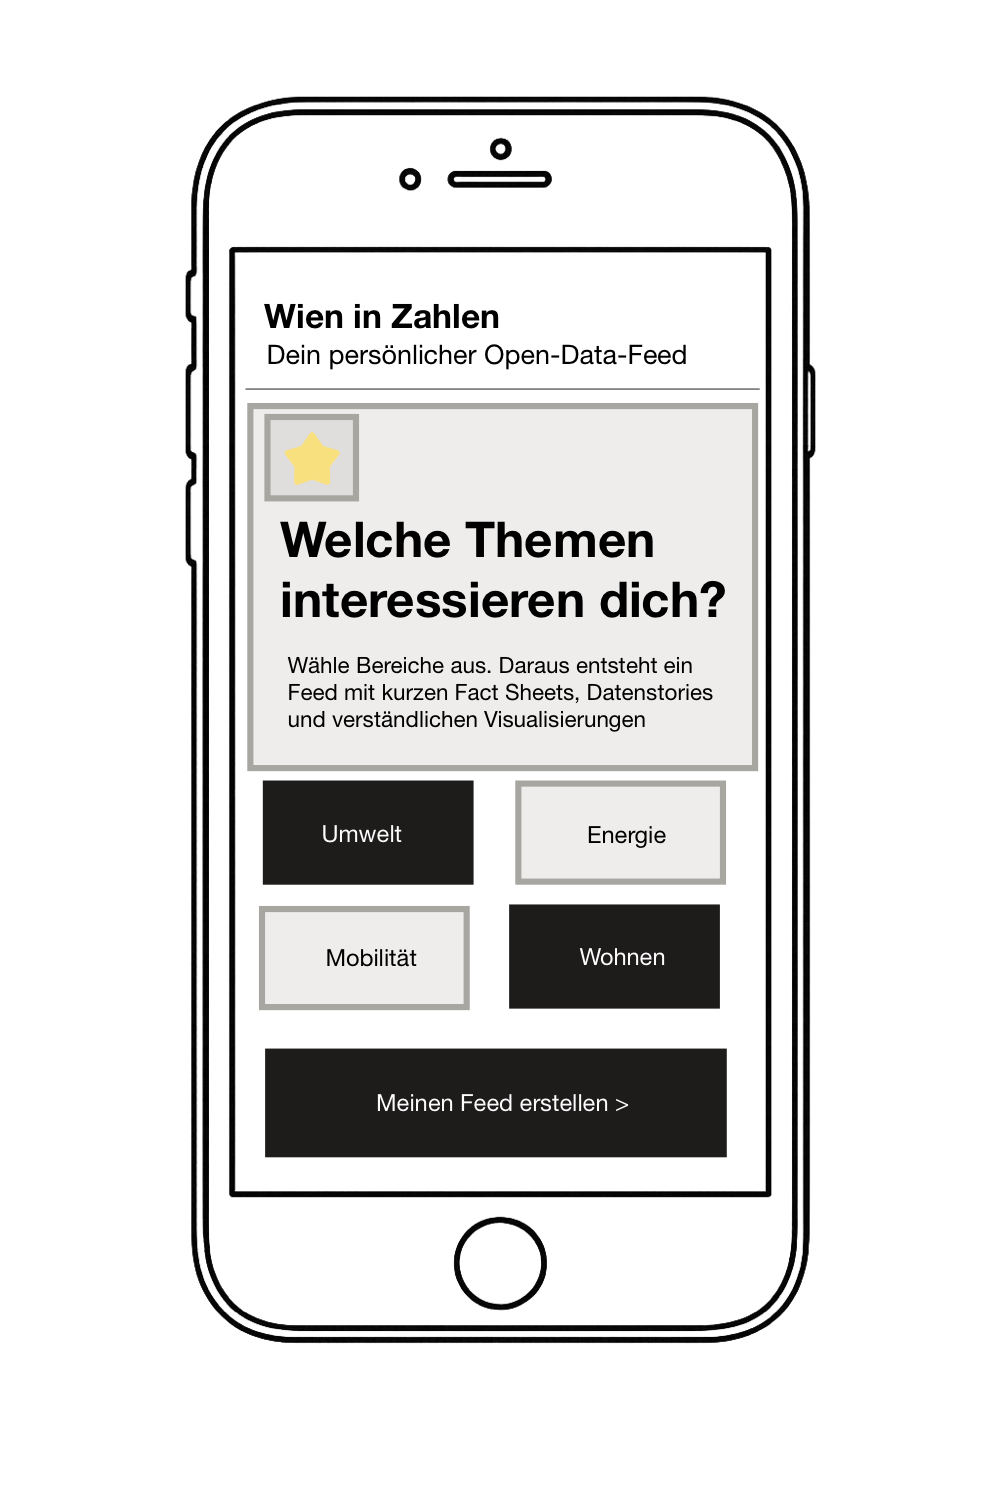
\includegraphics[width=0.25\textwidth]{../milestone_2/images/Feed_auswahl.png}
      }{
        \phantom{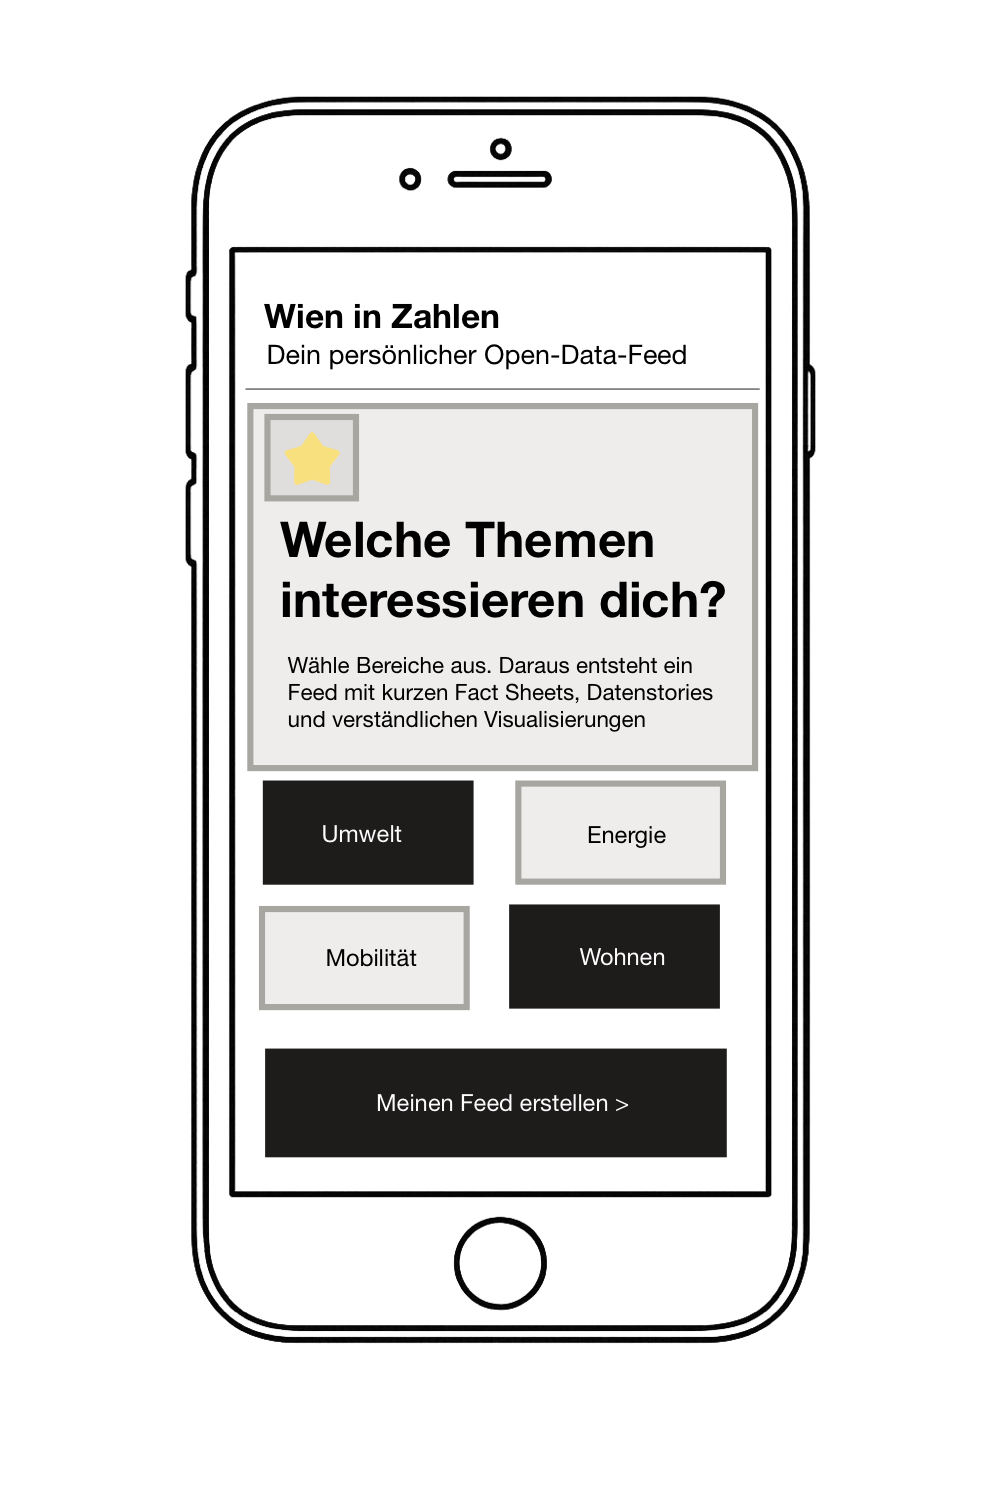
\includegraphics[width=0.25\textwidth]{../milestone_2/images/Feed_auswahl.png}}
      }
    };

    \node[img, right=of customization] (feed) {
      \alt<2->{
        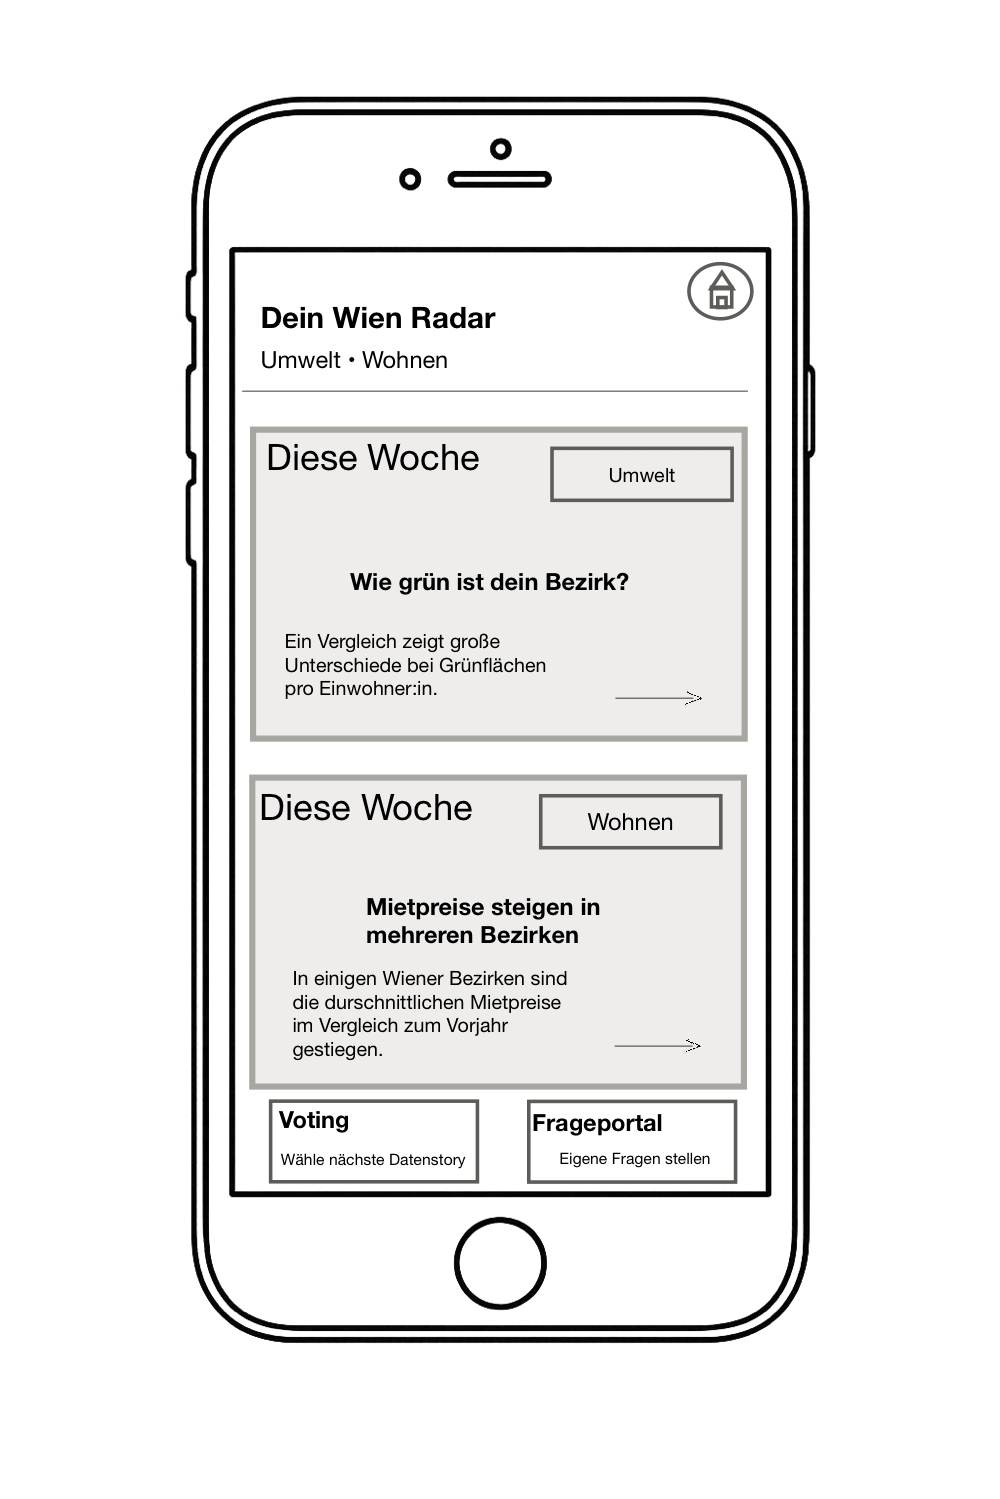
\includegraphics[width=0.25\textwidth]{../milestone_2/images/Feed.png}
      }{
        \phantom{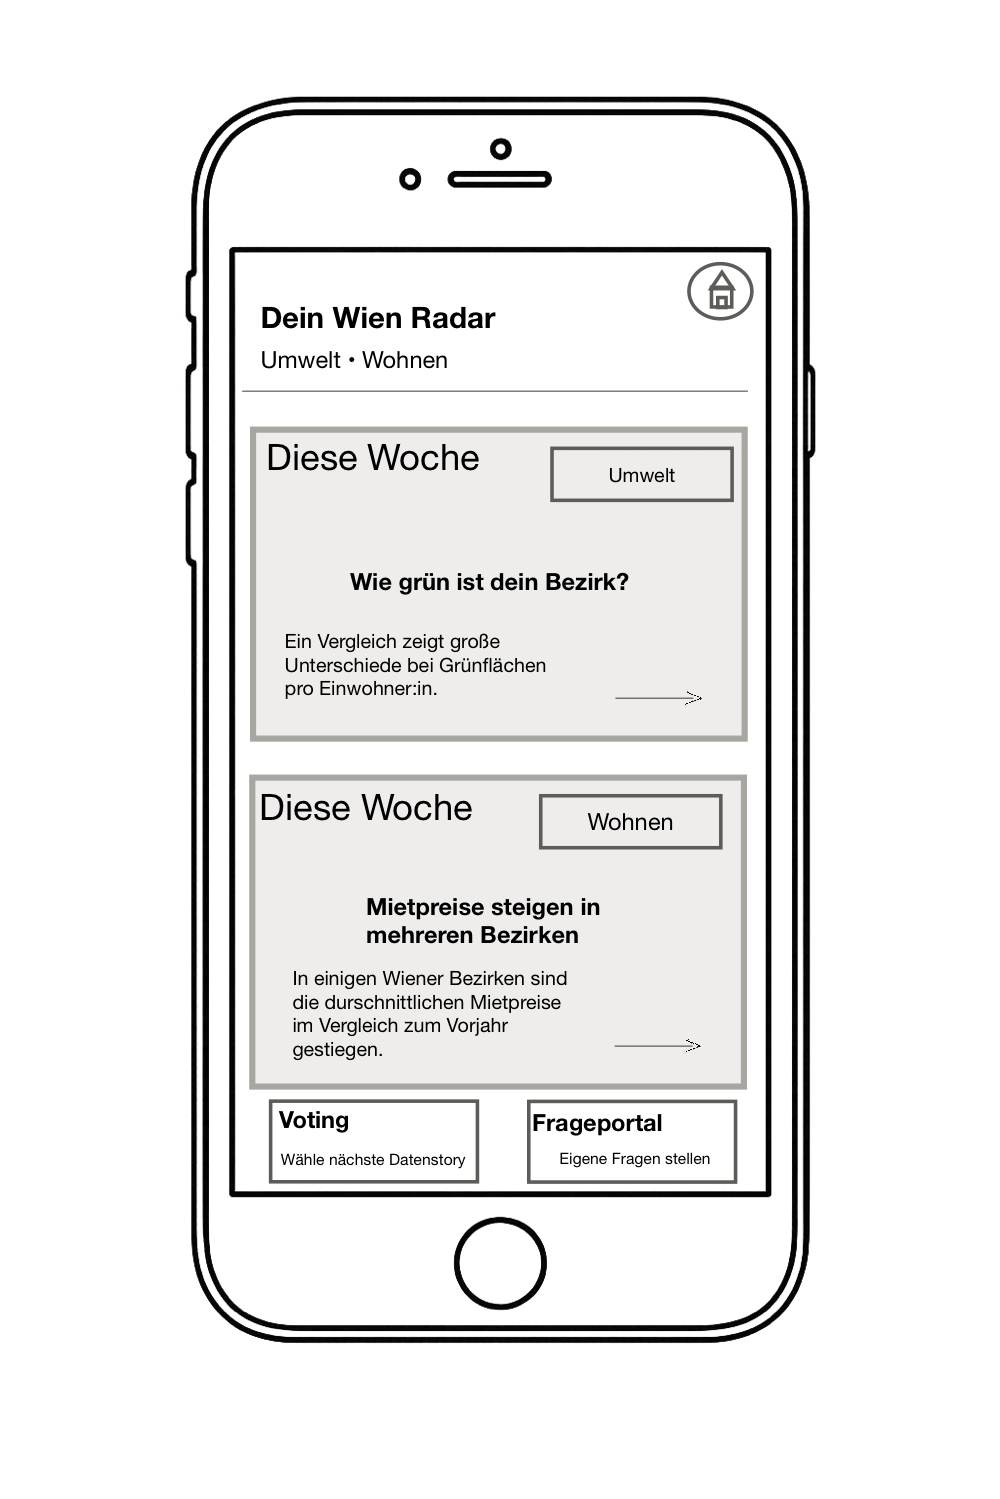
\includegraphics[width=0.25\textwidth]{../milestone_2/images/Feed.png}}
      }
    };

    \node[img, right=of feed] (factsheet) {
      \alt<3->{
        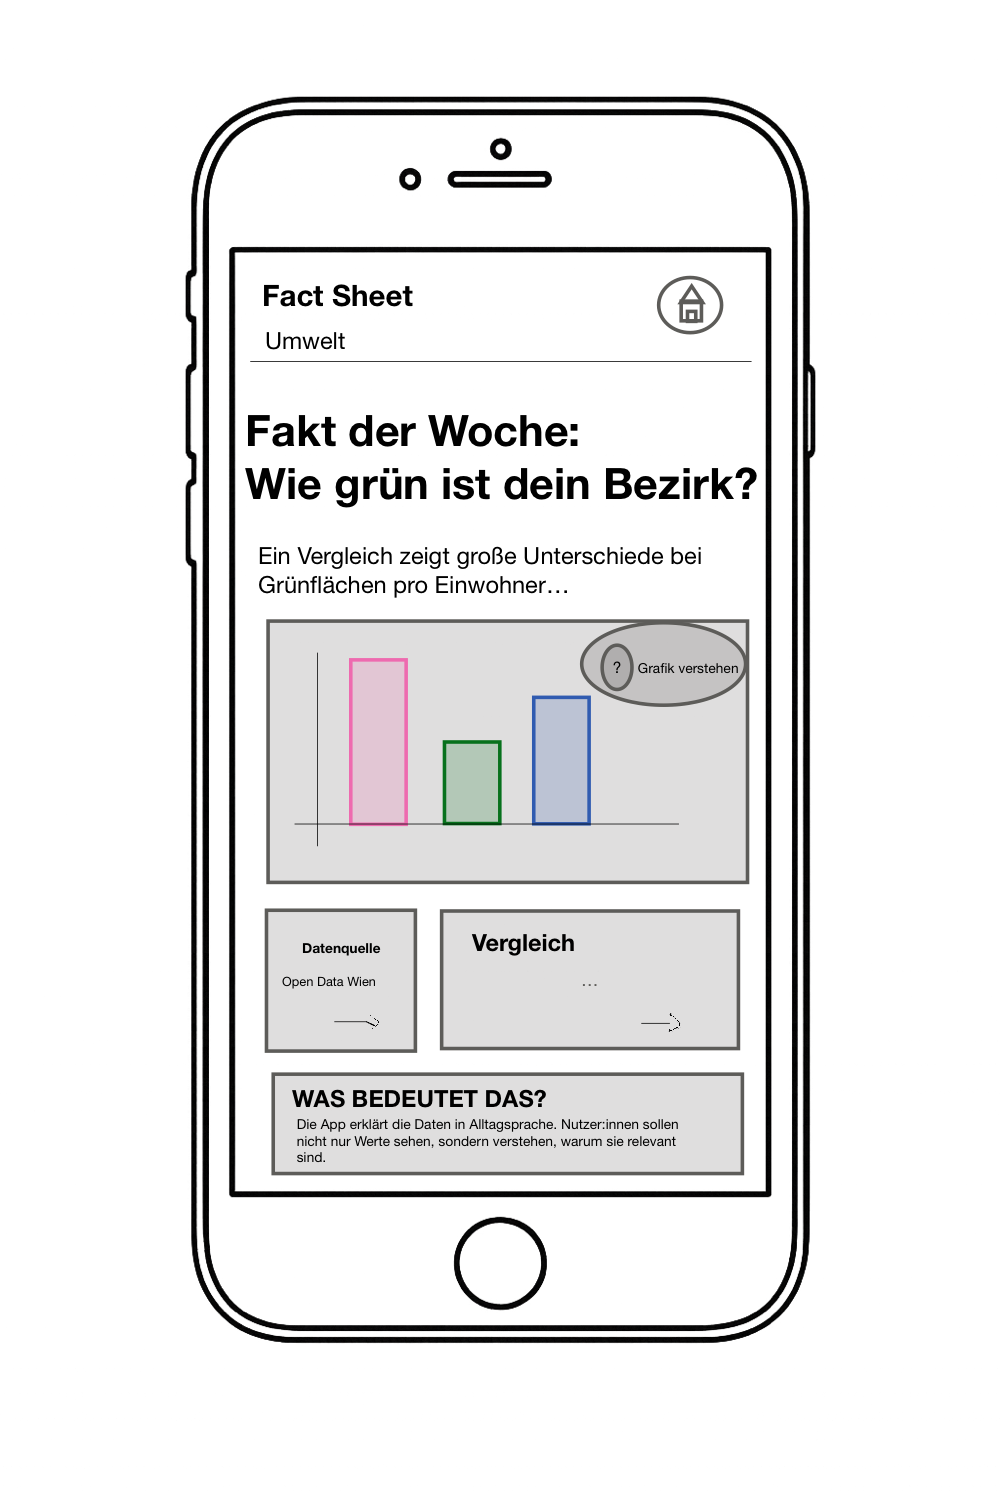
\includegraphics[width=0.25\textwidth]{../milestone_2/images/FactSheet.png}
      }{
        \phantom{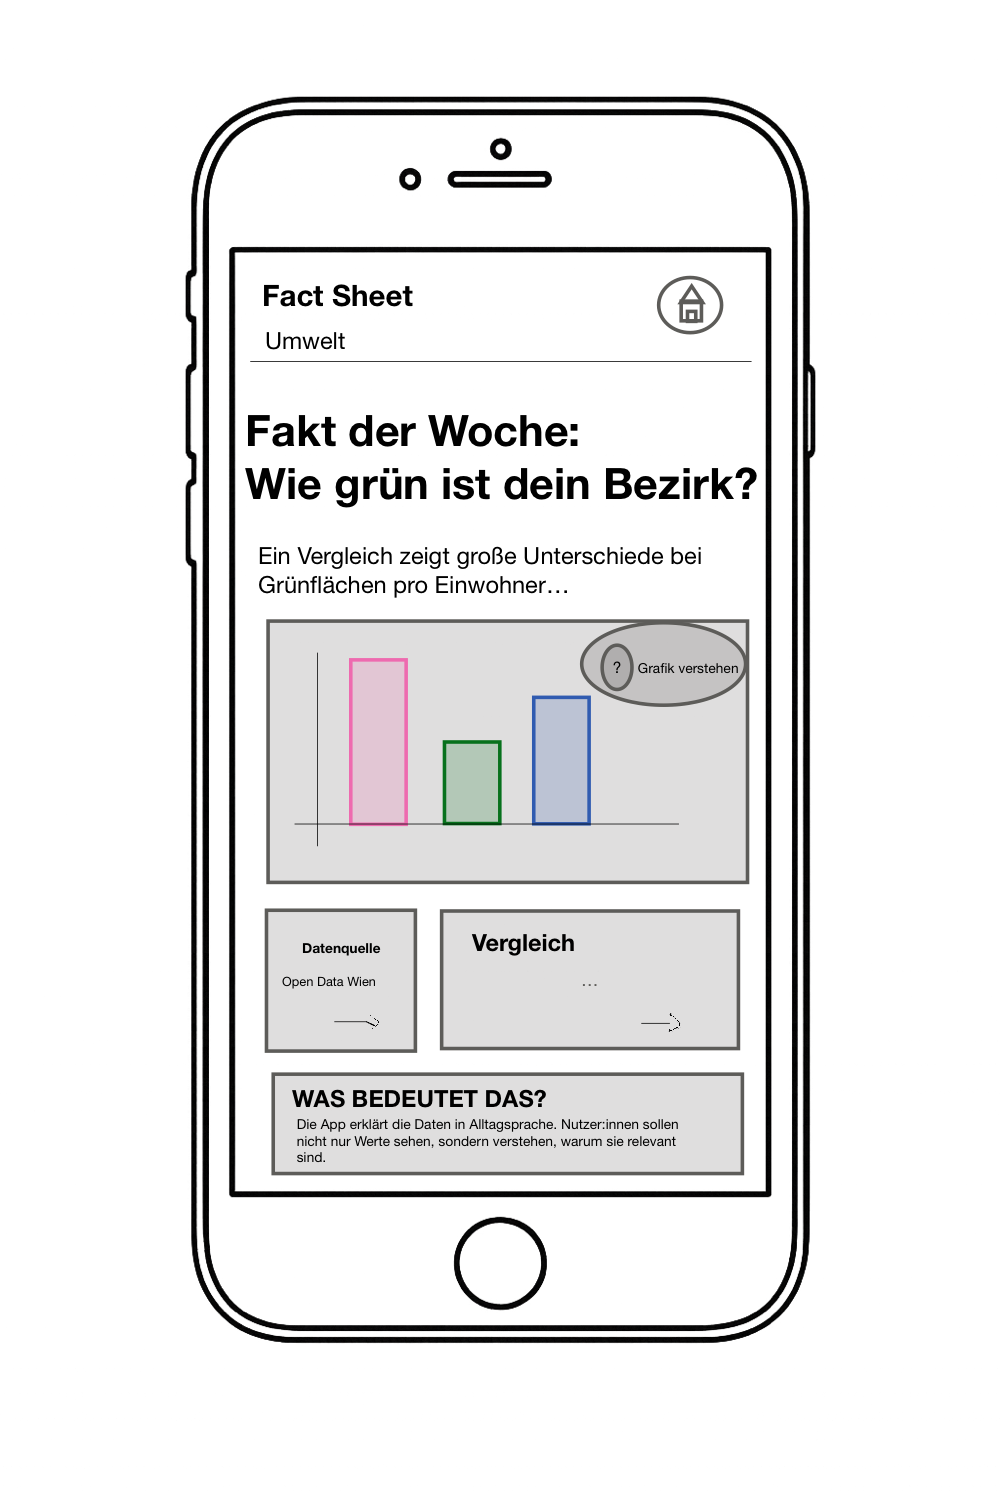
\includegraphics[width=0.25\textwidth]{../milestone_2/images/FactSheet.png}}
      }
    };

    % Pfeile erscheinen ebenfalls schrittweise
    \draw<2->[arrow] (customization.east) -- (feed.west);
    \draw<3->[arrow] (feed.east) -- (factsheet.west);

    % Beschriftungen
    \node[stepnum, below=0.18cm of customization] (s1) {
      \alt<1->{1}{\phantom{1}}
    };
    \node[captiontext, below=0.05cm of s1] {
      \alt<1->{Customization}{\phantom{Customization}}
    };

    \node[stepnum, below=0.18cm of feed] (s2) {
      \alt<2->{2}{\phantom{2}}
    };
    \node[captiontext, below=0.05cm of s2] {
      \alt<2->{Feed}{\phantom{Feed}}
    };

    \node[stepnum, below=0.18cm of factsheet] (s3) {
      \alt<3->{3}{\phantom{3}}
    };
    \node[captiontext, below=0.05cm of s3] {
      \alt<3->{Factsheet}{\phantom{Factsheet}}
    };

  \end{tikzpicture}

\end{frame}

\begin{frame}{Wien in Zahlen -- Anpassung}
  \centering
  \begin{minipage}{0.82\textwidth}
    \begin{itemize}
      \setlength\itemsep{0.85em}

      \item \textbf{Primäre Nutzer:innen:}\\
      Quellen, Vergleiche und Visualisierungen unterstützen Recherche, Analyse und schnelle Weiterverwendung.

      \item \textbf{Sekundäre Nutzer:innen:}\\
      Einfache Bedienung, kurze Texte und Erklärhilfen erleichtern den Einstieg.

      \item \textbf{Negative Persona:}\\
      Kontext, Interpretation und Quellen reduzieren missverständliche Nutzung.

    \end{itemize}
  \end{minipage}

\end{frame}

\begin{frame}{Wien in Zahlen -- Evaluierung}
  \alert{Durchführung:} Mitbewohner die low-Fidelity-Prototypen vorgestellt.

  \vspace{0.4cm}
  \alert{Fazit:}
  \begin{itemize}
    \item Unterschiedliche Zugänge zu Open Data positiv bewertet
    \item Verständlichkeit besonders wichtig
    \item Vertraute Abläufe wie Feed, Karte oder geführte Story hilfreich
  \end{itemize}
\end{frame}